\chapter{REVIEW OF LITERATURE AND STUDIES} \label{cap:chapter2}

% This chapter starts with a brief introductory paragraph concerning the researcher’s exploration of related literature and studies on the research problem. It should be organized thematically to confirm to the specific problems. It should synthesize evidence from all studies reviewed to get an overall understanding of the state of the knowledge in the problem area. As much as possible, the reviewed should be limited within the last ten years. A statement showing how the related materials had assisted the researchers in the present study should be the last part.  

% This chapter discusses the literature studies and theories of this study. It is divided into two sections: (1) the related literatures; and (2) the related studies.

% =========================================================
\section{Related Literatures}
% =========================================================
% This section discusses state of the art of Digital Forensics technologies and methods.
In previous studies, such as \citet{sylla2022secure}, the preventive aspect of reducing cheating in online exams conducted through Learning Management Systems (LMS) was discussed, including methods like using Secure Exam Browser (SEB) and randomizing questions. Meanwhile, the paper by \citet{ranger2020detection} focuses on detecting indicators of cheating in online exams.


A study of previous studies was done in order to better understand how forensic techniques are applied. The chosen papers examine a range of forensic techniques, such as proactive and reactive methods.

\begin{table}[H]
\centering
\caption{Overview of Research to Online Examination System and Forensic Technique}
\label{tab:literature-review}
\begin{tabular}{|p{2cm}|c|p{3cm}|p{2cm}|p{2cm}|p{4cm}|}
\hline
\textbf{References}        & \textbf{Year} & \textbf{Study Scope}                     & \textbf{Type of Forensics} & \textbf{Framework Used} & \textbf{Research Gap} \\ \hline
\citet{venter2018digital}  & 2018          & DFR on Online Examination                & Proactive Forensic         & ISO 27043:2015 & Using NIST 800-92 \\ \hline
\citet{kadoic2018analysis} & 2018          & Moodle usage and academic success on student behaviour analysis logs-based   & Not forensic purpose         & None         & Using logs-based for forensic activity   \\ \hline
\citet{rivera2019towards}  & 2019          & Forensic-ready logging systems           & Proactive Forensics        & OWASP & Using framework logging by NIST 800-92 \\ \hline
\citet{febriana2023comparative} & 2023          & Integrating Forensic Techniques into Incident Response in private cloud                   & Reactive        &  NIST 800-86 and ISO 27043:2015 & Difference environment on scope academic and using logging by nist 800-92      \\ \hline
\citet{lakhno2023adaptive}  & 2023 & Information System Security & Proactive Forensic & NIST 800-92 & DIfference environment by academic purpose online exam \\ \hline
\citet{kern2024logging}    & 2024 & Logging maturity & Proactive and Reactive Forensic & NIST 800-53 & Using nist 800-92 \\ \hline
\citet{abd2024enhancing}   & 2024          & LMS with forensic logging                & Proactive Forensics        & Using framework by owasp describe 5W+1H & Using framework by NIST 800-92 for logging management    \\ \hline
\citet{lintang2024log}     & 2024          & LMS activity during online tests         & Proactive Forensics        & None  & using framework by nist 800-92 for proactive forensic purpose     \\ \hline
\end{tabular}
\end{table}

The table \ref{tab:literature-review} shows that different methodological techniques are employed to enable proactive forensics. To find research gaps that can be the basis for creating a proactive log management framework based on forensics, a comparison analysis has also been carried out. The main goal is to combine log management techniques that improve preventive evidence loss with suggestions from the NIST 800-92 framework.


As an aspect I aim to develop from previous research, the lack of forensic readiness preparedness has been identified. Therefore, as shown in the image below, this represents the framework I have developed.

\begin{figure}[H] 
    \centering
    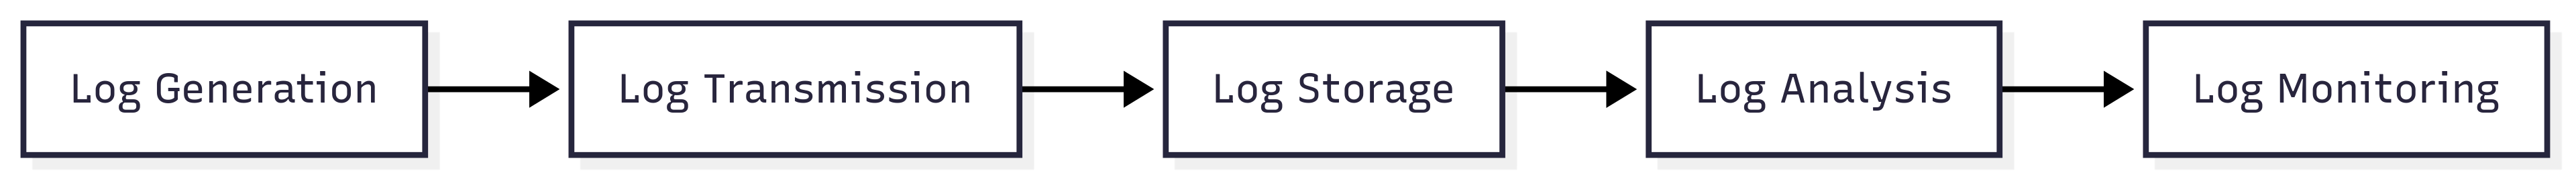
\includegraphics[width=14cm]{figure/log-management-nist-800-92-original.png}
    \caption{ Phase log management from NIST 800-92}
    \label{fig:nist-log-management}
\end{figure}


\begin{itemize}
    \item \textbf{Log Generation:} The process where logs are created by operating systems, applications, and network devices to record events or activities.
    \item \textbf{Log Transmission:} The step where generated logs are transmitted to centralized storage or log management systems, either in periodically.
    \item \textbf{Log Storage:} Logs are stored in a secure and organized manner, ensuring availability, confidentiality, and integrity for future analysis.
    \item \textbf{Log Analysis:} Stored logs are analyzed to identify patterns, detect anomalies, investigate incidents, or support forensic investigations.
\end{itemize}


% =========================================================
\section{Related Studies}
% =========================================================
% This section discusses about the related studies which support in the designing of the proposed method.
This section explores related studies that underpin the proposed method's design.

\subsection{Digital Forensics}  Digital forensics, also known as computer forensics, encompasses a wide spectrum of forensic investigations that extend beyond traditional computer devices. It incorporates expertise from various domains, including network forensics, database forensics, mobile device forensics, cloud forensics, memory forensics, and data or disk forensics.\cite{paul2019analysisdf}.

The digital forensic process has several general stages, such as, identifying, preservation, analysis and presentation. these phases were proposed by mckemmish in 1999.

\textbf{Proactive Forensics}: the ability to proactively collect, trigger an
event, and preserve and analyze evidence to identify an incident as it occurs. In addition, an automated preliminary report is generated for a later
investigation by the reactive component. Proactive evidence pertaining to
a particular occurrence or incident as it happens will be acquired in this
component \cite{proactiveandreactivedigitalforensics}

\textbf{Reactive Forensics}:  the conventional method of looking into
a digital crime after it has happened, often known as the post-incident
method \cite{proactiveandreactivedigitalforensics}. Identification, preservation, collection, analysis, and production of the final report are all part of this process.

\begin{figure}[H] 
    \centering
    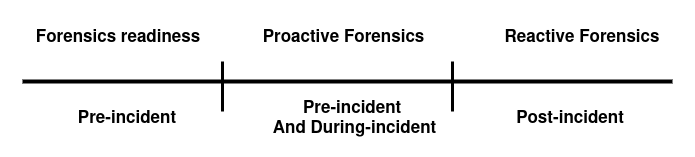
\includegraphics[width=14cm]{figure/flow-fr-pro-react.jpg}
    \caption{Forensic Readiness, Proactive Forensics and Reactive Forensic }
    \label{fig:fr-pro-reac}
\end{figure}

\textbf{Fig} \ref{fig:fr-pro-reac} above there is several section from forensic readiness, proactive forensics and reactive. The three methods mentioned above have a distinction in their application when dealing with cybercrime.

\begin{figure}[H] 
    \centering
    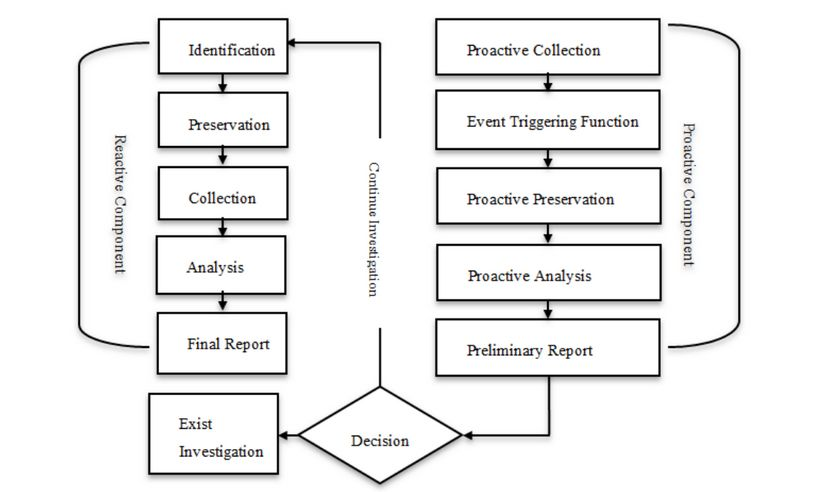
\includegraphics[width=14cm]{figure/proactive-reactive-flow-process.jpg}
    \caption{Functional process for proactive and reactive digital forensics investigation system \cite{proactiveandreactivedigitalforensics}}
    \label{fig:flow-pro-react}
\end{figure}

In \textbf{Fig} \ref{fig:flow-pro-react} Explain flow process the differences reactive and proactive forensics. Proactive collect the logs before the incident occured.

\begin{itemize}
    \item \textbf{Proactive Collection} : Automated live collection of a pre-defined data in the order
of volatility and priority, and related to a specific requirement of an organization.
    \item \textbf{Even Triggering Function} : Suspicious event that can be triggered from the
collected data.
    \item \textbf{Proactive Preservation} : Automated preservation of the evidence related to the
suspicious event, via hashing.
    \item \textbf{Proactive Analysis} : automated live analysis of the evidence, which might use
forensics techniques such as data mining to support and construct the initial
hypothesis of the incident.
    \item \textbf{Preliminary Report}: Automated report for the proactive component. 
\end{itemize}

Reactive methods struggle to identify and prove attacks efficiently. Proactive methods solve this by enabling real-time investigations and organizing data to save time and space. This makes proactive approaches faster and more effective for forensic investigations\cite{SPNFFb16}.
\subsection{Log Management} Effective log management practices are critical for maintaining computer security records with the necessary detail and for an appropriate retention period, as outlined in NIST Special Publication 800-92 (SP 800-92). Additionally, log analysis proves beneficial for auditing, 
forensic analysis, internal investigations, establishing baselines, and identifying operational trends and long-term problems. \cite{kentnist800922006guide}

The log management process encompasses a series of sequential steps, as outlined below:
\begin{enumerate}
\item \textbf{Log Generation:} The process where systems or devices generate logs. Logs can be created by various sources such as firewalls, servers, applications, etc. These logs record events, transactions, or activities that provide valuable information for security monitoring and auditing.

    \item \textbf{Log Transmission:} The process of sending logs from the source (e.g., firewall, server, application) to a central storage or analysis system. This can be done via various methods, such as syslog, agent-based collection, or secure transmission protocols to ensure the integrity and confidentiality of the data.

    \item \textbf{Log Storage:} The phase where logs are stored either in raw or structured formats. This could include storage in flat files, databases, or Security Information and Event Management (SIEM) systems. Proper storage ensures that logs are easily accessible for future analysis, audits, and incident investigations while maintaining their integrity.

    \item \textbf{Log Analysis:} The phase of examining logs to detect anomalies, patterns, or security incidents. This involves using automated tools or manual review to identify suspicious activities, potential threats, or system malfunctions. Log analysis helps in proactive threat detection and reactive forensics during security incidents.
\end{enumerate}

\subsection{Learning Management System} Learning Management Systems (LMS) create virtual classrooms that enhance learning for both instructors and students.  These online environments provide a framework for fostering an inclusive learning experience that supports academic progress. LMS tools encourage collaboration among students through online groups, discussions, and communication features, extending the benefits to all users \cite{bradley2021learninglms}. 

Numerous studies have been conducted to evaluate and develop LMS. Smith and Brown~\cite{smith2020} conducted a comparative study between Moodle and Google Classroom in higher education institutions. The study found that Moodle offers more features supporting structured learning processes, while Google Classroom is easier to use for both instructors and students.

Another research by Wijaya \textit{et al.}~\cite{wijaya2021} investigated the use of mobile-based LMS in distance learning. Their study found that the use of mobile-based LMS can increase student participation, especially during online learning in the COVID-19 pandemic.

Furthermore, Putra and Sari~\cite{putra2022} explored the integration of artificial intelligence technology into LMS. The results indicated that AI-based recommendation systems in LMS can help improve students' motivation and engagement in the learning process.

However, most existing studies are still limited to aspects of usability and features, while issues related to scalability and data security in LMS for large-scale institutions have not been widely discussed~\cite{kumar2019}.
